\documentclass{beamer}
\usepackage{listings}

\title{Implementation and comparison of local search algorithms applied to the eight queens puzzle}

\author{Francesco Esposito}

\institute {
  Faculty of Computer Engineering \\
  Università degli studi di Napoli ``Federico II"
}

\date{June 2024}
    
\begin{document}
    \frame{\titlepage}
    
    \begin{frame}
    \frametitle{Introduction}
        \begin{itemize}
            \item Goal: Solve eight queen puzzle using different local search algorithms.
            \pause
            \begin{itemize}
                \item Proprieties and performance of algorithms are also discussed.
            \end{itemize}
            \pause
            \item How? Using Python for the implementation and ``Artificial Intelligent: A Modern approach (third edition)" as a reference.
            \pause
            \begin{itemize}
                \item Code will be available on Github (on francespos account) after the exam.
            \end{itemize}
        \end{itemize}
    \end{frame}

    \begin{frame}
    \frametitle{The eight queens puzzle}
        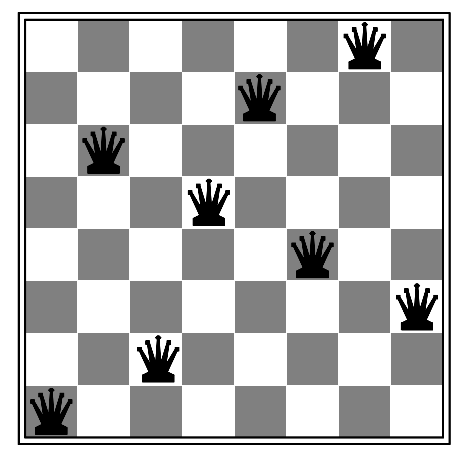
\includegraphics[scale=0.5]{Images/8_queens_puzzle.png}
        \centering
    \end{frame}

    \begin{frame}
    \frametitle{The eight queens puzzle}
    \begin{itemize}
        \item Problem: place eight queens on a chessboard so that they don't attack each other.
        \pause
        \item Rules: A queen can move horizontally, vertically and diagonally within an arbitrary range.
        \pause
            \begin{itemize}
                \item We will ignore states where queens are on the same column, because they can't belong to the solution.
            \end{itemize}
        \pause
        \item We will use PEAS approach to describe the problem.
    \end{itemize}
    \end{frame}

    \begin{frame}
    \frametitle{PEAS}
        \begin{itemize}
            \item Performance measure: (Opposite of) number of pairs of queens that attack each other.
            \pause
            \item Environment: 8x8 chessboard with eight queens. 
            \pause
            \item Actuator: Player who moves the queens.
            \pause
            \item Sensor: Player looking at the board.
        \end{itemize}
    \end{frame}

    \begin{frame}
    \frametitle{State space representation}
        \begin{itemize}
            \item Since a column must be occupied by a single queen, we will represent states as a list of eight numbers between 0 and 7.
            \pause
            \begin{itemize}
                \item The element in position i is the row position of the queen on column i.
            \end{itemize}
        \end{itemize}
    \end{frame}

    \begin{frame}
    \frametitle{State space representation}
        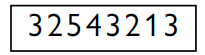
\includegraphics{Images/queens_position.png}
        \centering
    \end{frame}

    \begin{frame}
    \frametitle{Adjacent state: implementation}
        \begin{itemize}
            \item An adjacent state corresponds to a movement of a queen in her column.
            \pause
            \item For each column c (i.e. position in the list), for each row r (i.e. value of an element in that position): 
            \pause
            \begin{itemize}
                \item if queen in the column c is not in position r, an adjacent state is represent by the same list with the new element r in position c.
            \end{itemize}
        \end{itemize}
    \end{frame}

    \begin{frame}
    \frametitle{Heuristic function: implementation}
    \begin{itemize}
        \item An heuristic function is the number of pairs of queens that attack each other.
        \pause 
        \item This heuristic function is admissible, because it never overestimates the cost of reaching the goal.
        \pause
        \begin{itemize}
            \item To resolve n conflicts, at least n moves are required.
        \end{itemize}
        \pause
        \item The heuristic function is calculated as the number of conflicts on each row and on each diagonal.
    \end{itemize}
    \end{frame}

    \begin{frame}
    \frametitle{Hill climbing: implementation}
        \begin{itemize}
            \item Hill climbing search algorithm only stores the current state.
            \pause
            \item In each iteration, it moves to the adjacent state with the lowest value.
            \pause
            \begin{itemize}
                \item In other words, it points to the direction of the steepest descent.
            \end{itemize}
            \pause
            \item Starting from initial state, the heuristic function is assessed for each neighbor, and the state with the lowest value is chosen.
            \pause
            \begin{itemize}
                \item After an iteration, we get a pair (state, value) for the best neighbor.
                \pause
                \item If ``value" is greater than or equal to current state value, a local minimum has been reached.
                \pause
                \item Otherwise, a new iteration starts with the pair (state, value).
            \end{itemize} 
        \end{itemize}
    \end{frame}

    \begin{frame}
    \frametitle{Hill climbing: Properties}
     \begin{itemize}
         \item Complete? \pause No.
         \pause The algorithm is ``greedy", because he chooses a nearby good state without considering the further states.
         \pause
         \item Time? \pause 
         \begin{math}O(n^2).\end{math}
         \pause The number of neighbors of a queen is \begin{math}n-1\end{math}, so the total number of adjacent states is \begin{math}n * (n-1)\end{math}.
         \pause
         \item Space? \pause
         \begin{math}O(1).\end{math}
         \pause Only the current state is stored.
     \end{itemize}   
    \end{frame}

    \begin{frame}
    \frametitle{Simulated annealing: implementation}
    \begin{itemize}
        \item Simulated annealing chooses a random move, rather than the best one.
        \pause
        \item If the move improves the heuristic value, it will always be choose, otherwise it is accepted with some probability p \begin{math}< 1\end{math}.
        \pause
        \item Probability exponentially decreases with the worsening of the heuristic value and the lowering of temperature.
        \pause
        \item If temperature decreases slowly, for the Boltzmann distribution propriety, all probability is centered on global minimum with a limit value of 1.
    \end{itemize}
    \end{frame}

    \begin{frame}
    \frametitle{Simulated annealing: Properties}
     \begin{itemize}
         \item Complete? \pause No. \pause Simulated annealing uses a probabilistic model. To reach completeness, theoretically,  cooling should be infinitely slow.
         \pause
         \item Time? \pause 
         \begin{math}O(t)\end{math}, where t is the cooling speed.
         \pause
         \item Space? \pause
         \begin{math}O(1).\end{math}
     \end{itemize}   
    \end{frame}

    \begin{frame}
    \frametitle{Genetic algorithm: implementation}
        \begin{itemize}
            \item Genetic search algorithms are built on the theory of natural selection: in each generation, the best individual are selected for reproduction.
            \pause
            \begin{itemize}
                \item In each generation, individuals reproduce with a probability that depends on their fitness value.
            \end{itemize}
            \pause
            \item The recombination procedure occurs by randomly selecting a crossover point, at which the parents are divided to form their children.
        \end{itemize}
    \end{frame}

    \begin{frame}
    \frametitle{Genetic algorithm: Properties}
     \begin{itemize}
         \item Complete? \pause No.
         \pause         
         Genetic algorithms are also based on probabilistic models.
         \pause
         \item Time? \pause 
         \begin{math}O(km)\end{math}, where k is the maximum number of iterations and m is the population size.
         \pause
         \item Space? \pause
         \begin{math}O(m).\end{math} 
         \pause
         The current population is stored.
     \end{itemize}   
    \end{frame}
\end{document}